\documentclass[12pt, letterpaper]{article}
\usepackage[utf8]{inputenc}
\usepackage[english]{babel}
\usepackage{fancyhdr}
\usepackage{geometry}
%\usepackage{natbib}
\usepackage{indentfirst} % to indent the first paragraph after a section heading
\usepackage{apacite}
\bibliographystyle{apacite-copy}
%\setcitestyle{aysep={,}} % separate author name and year with a comma
\renewcommand{\BRetrievedFrom}{" "}
\renewcommand{\BRetrieved}{" "}
\renewcommand{\doiprefix}{https://doi.org/}

\usepackage{booktabs, tabularx, longtable}
\usepackage{array}
\usepackage{colortbl}
\usepackage{graphicx}
\usepackage[section]{placeins}
\usepackage{amsmath}
\usepackage[leftcaption]{sidecap}
\graphicspath{ {./figures/} }
\usepackage{setspace}
\usepackage{caption}
\captionsetup[table]{font={stretch=1.05, small}}   %% change table caption spacing
\captionsetup[figure]{font={stretch=1.05, footnotesize}} %% change figure caption spacing
\usepackage{titlesec}
\titleformat{\section}
 {\normalfont\fontsize{14}{15}\bfseries}{\thesection}{1em}{} %change the size of section header font
\titleformat{\subsection}
 {\normalfont\fontsize{12}{15}\bfseries}{\thesubsection}{1em}{} %change the size of subsection header font
\renewcommand{\thesection}{} %remove the section numbers
\renewcommand{\thesubsection}{} %remove subsection numbers

%try to deal with the problem of too long figure caption
\DeclareCaptionLabelFormat{adja-page}{\hrulefill\\#1 #2 \emph{(previous page)}}
\usepackage{subfig}

%try to deal with issue of figures going to the end of the document
\makeatletter
\AtBeginDocument{%
 \expandafter\renewcommand\expandafter\subsection\expandafter{%
  \expandafter\@fb@secFB\subsection
 }
}
\makeatother

\geometry{margin = 1in}
\pagestyle{fancy}
\fancyhf{}
%set the header
\rhead{\thepage}
\lhead{A. Stears}
%set the line spacing
\renewcommand{\baselinestretch}{2}
%add line numbers
\usepackage{lineno}
\linenumbers


%\title{Demographic trade-offs affect how leaf turgor loss point and tissue dry matter content mediate the effect of drought on herbaceous perennial survival and growth} 
%\author[1]{Alice Stears}
%\author[2]{Peter Adler}
%\author[3]{Dana Blumenthal}
%\author[3]{Julie Kray}A demographic trade-off determines how Leaf turgor loss point and tissue dry matter content mediate the effect of drought on herbaceous perennial survival and growth
%\author[4]{Troy Ocheltree}
%\author[5]{Kevin Wilcox}
%\author[1]{Daniel C. Laughlin}

% Include full affiliation details for all authors
%\affil[1]{Botany Department and Program in Ecology, University of Wyoming, Laramie, WY}
%\affil[2]{Department of Wildland Resources and the Ecology Center, Utah State University, Logan, UT}
%\affil[3]{USDA-ARS Rangeland Resources Research Unit, Fort Collins, CO}
%\affil[5]{Department of Ecosystem Science and Management, University of Wyoming, Laramie, WY}
%\affil[4]{Warner College of Natural Resources, Colorado State University, Fort Collins, CO}

\begin{document}

\begin{flushleft}
\Large{\textbf{Functional traits predict demographic responses to drought in a semiarid shortgrass steppe}} 

\normalsize{Alice E. Stears$^{1*}$, Peter B. Adler$^2$, Dana M. Blumenthal$^3$, Julie A. Kray$^3$, Kevin E. Mueller$^4$, Troy W. Ocheltree$^5$, Kevin R. Wilcox$^6$, Daniel C. Laughlin$^1$}

\small{$^1$Botany Department and Program in Ecology, University of Wyoming, Laramie, WY; \linebreak
$^2$Department of Wildland Resources and the Ecology Center, Utah State University, Logan, UT; \linebreak
$^3$USDA-ARS Rangeland Resources Research Unit, Fort Collins, CO; \linebreak
$^4$Department of Biological, Geological and Environmental Sciences, Cleveland State University, Cleveland, OH; \linebreak
$^5$Warner College of Natural Resources, Colorado State University, Fort Collins, CO; \linebreak
$^6$Department of Ecosystem Science and Management, University of Wyoming Laramie, WY}\linebreak

\small{$^*$Corresponding Author: astears@uwyo.edu}

\small{
\textbf{Author Contributions}: AES and DCL contributed to study conception and design. DMB, JAK, KEM, TWO, and KRW collected trait data, and PBA collected demographic data. Analysis was performed by AES with contributions from DCL, DMB, and PBA. AES wrote the manuscript with contributions from all authors. 
} 

\small{\textbf{Data Availability Statement}: All data and code that has not previously been published will be available from Dryad. }

\end{flushleft}
\textbf{Keywords:} demographic rates, drought, functional traits, global change, grasslands, vital rates

\begin{abstract}
\begin{enumerate}


\item Characterizing how plant traits mediate demographic responses to abiotic conditions may provide a mechanistic explanation of species responses to environmental variation. This is critical for understanding how drought, which will become more frequent and intense with global change, impacts plant communities and ecosystem services. We predicted that (1) species with low leaf turgor loss point (TLP) and high leaf and root dry matter content (LDMC and RDMC) would be more likely to survive and grow in dry years because of higher wilting resistance, and (2) these traits would more weakly predict growth and survival in wet years. (3) Traits related to water use that most directly measure physiological mechanisms would predict demographic responses better than morphological traits unrelated to water use.
\item We synthesized 15 years of demographic data, species-level functional trait measurements, and climate records in a shortgrass steppe ecosystem in Colorado. We fit generalized linear mixed effect models to determine whether traits interact with drought to impact growth and survival while accounting for plant size and local intraspecific competition.
\item Plant size positively affected survival, and local intraspecific competition negatively affected growth and survival across all species. Graminoids with more negative TLP and higher LDMC and RDMC had higher survival rates in dry years. However, graminoids with less negative TLP and lower LDMC and RDMC were larger than species with high TLP, low LDMC and RDMC, in both wet and dry years. Forbs demonstrated similar yet more variable responses to drought.
\item \textit{Synthesis} Traits that dictate the nature of a plant’s physiological response to drought mediate the effects of abiotic variation on demographic rates. Traits significantly mediated the impact of drought on survival, but not on growth, indicating that survival could be the primary demographic driver of species' drought response in this system. The physiological trait TLP was a good predictor of survival in response to drought, but the easier-to-measure morphological traits LDMC and RDMC were equal or better predictors. These results advance our understanding of the mechanisms by which drought drives plant population dynamics, and will refine our predictions of how plant communities will respond to more intense and frequent drought.
\end{enumerate}
\end{abstract}

\section{Introduction}
As the frequency and intensity of extreme weather events increases with climate change, it becomes increasingly important to understand how plant populations and communities will respond \shortcite{Vicente-Serrano2020AWarming}. Climate models predict that some regions will receive more precipitation in concentrated extreme-precipitation events, while other regions will receive less moisture overall with longer periods of more extreme drought between precipitation events \cite{Knapp2008ConsequencesEcosystems}. While climate models struggle to predict fine-scale variation in precipitation, most models indicate that western North America will undergo more frequent and intense drought as climate change progresses \cite{Hartmann2013}.

Environmental variation affects plant growth, survival, and reproduction, and these impacts are primarily mediated through the phenotype of a plant, which can be quantitatively characterized by functional trait values \shortcite{Laughlin2020TheFitness}. In order to improve our understanding of how plant populations and communities respond to climate change, it is useful to define how plant traits mediate the effect of environmental variation on plant fitness, and to identify the traits that are relevant to this process for different abiotic stressors. Previous work has characterized variation in community-level trait values along gradients of aridity. Both experimentally-induced and naturally-occurring gradients of water availability drive shifts in community-weighted mean (CWM) trait values. For example, drier communities have lower CWM-SLA \cite{Nunes2017WhichDrylands, Cornwell2009CommunityCalifornia}. And in these dry communities, higher SLA species increase in abundance in wet years \cite{Wilcox2020PlantPrairie}. Other studies observed little to no variation in CWM traits after drought, but have identified either decreased functional diversity (FD) in dry sites \cite{Luo2019LongGrasslands} or increased FD immediately after experimentally-induced drought \cite{Griffin-Nolan2019}. In North American shortgrass steppe, plant species with low leaf osmotic potential (a primary determinant of turgor loss point \cite{Bartlett2012a}), high leaf dry matter content (LDMC) and low SLA are relatively insensitive to interannual precipitation variability \cite{Wilcox2020PlantPrairie}. In the same ecosystem, correlations among these and other traits indicate tradeoffs between drought resistance and rapid resource acquisition and use \cite{Blumenthal2020}. Additional work in dry a California grassland has found that species with traits correlated with a conservative resource acquisition strategy such as lower growth rate and higher leaf lobedness are more likely to survive drought \cite{Luong2021}. Determining how these traits affect growth and survival of individual plants can help provide a mechanistic understanding of plant population responses to interannual variation in weather, as well as improve our understanding of drought-tolerance mechanisms in grassland plants.

Individual-level impacts of abiotic variation are observed first in the physiological responses of plants to stress, such as wilting in response to decreased water availability (Bartlett, Scoffoni, Ardy et al., \citeyearNP{Bartlett2012}, Bartlett et al., \citeyear{Bartlett2016TheDrought}). After a plant’s physiological ability to withstand or escape drought is surpassed, death or decreased fecundity negatively impacts population sizes for more drought-susceptible species \cite{Koerner2014}. Community composition may then be altered, in turn altering the competitive and facilitative interactions between individuals within that community \cite{Ploughe2019CommunityInteractions, Harrison2015Climate-drivenCommunity}. In extreme cases, this process can lead to either species extirpation or recruitment of formerly absent species to the local species pool, changing both the functional and phylogenetic diversity of the plant community. Evaluating the underlying demographic mechanisms and plant-plant interactions that are driving community dynamics is an important next step in functional, population, and community ecology, and will allow us to predict how plant phenotypes mediate the impacts of extreme climate plant demographic rates \shortcite{Laughlin2020TheFitness, Ploughe2019CommunityInteractions, Hoover2014ResistanceExtremes, Salguero-Gomez2012}.

In order to isolate the importance of plant traits for whole-plant responses to drought, we must first account for factors unrelated to functional traits that impact how plants respond to abiotic conditions. First, individuals are more likely to survive to the next year if they are larger and more established than smaller individuals of the same species \shortcite{Tredennick2017}. Second, competition and facilitation between individuals can have correspondingly negative and positive impacts on demographic rates \shortcite{Adler2012}. Even after accounting for these known drivers of demography, we lack a general understanding of which traits interact with drought to drive plant demographic rates, and thus fitness \shortcite{Laughlin2018, Laughlin2020TheFitness}(Fig. \ref{fig:ConceptFig}).  

While definitions of "functional traits" abound \shortcite{Violle2007, Volaire2020WhatProcesses, Mcgill2006}, a majority of trait-based studies focus on a similar set of traits, specifically leaf economic traits such as specific leaf area (SLA) \shortcite{Wright2004, Reich2014} and root economic traits such as root tissue density \cite{Kramer-Walter2016}. These economic traits are correlated with each other along an axis that represents resource acquisition strategy, falling on a spectrum from fast (e.g. high SLA, low LDMC) to slow (e.g. low SLA, high LDMC). Economic trait values indicate a plant’s strategy for acquiring any limiting resource, including carbon, nutrients, and water \cite{Reich2014}. We measured SLA, LDMC, and RDMC, economic traits that are correlated with plant relative growth rate and resource-acquisition strategy \cite{Weiher1999ChallengingEcology}. We expect that LDMC, in particular, is relevant to a plant’s ability to acquire water under drought conditions because it is a more direct measurement of leaf structure and allocation of carbon to leaf tissue than SLA \cite{Niinemets1999ComponentsPlants, Hodgson2011}. Species with higher LDMC have higher allocation to cell wall structure and more densely-packed leaf cells, and thus are more likely to maintain cell turgor under water stress \cite{Niinemets2001Global-scaleShrubs, Poorter2009CausesMeta-analysis, Wilcox2020PlantPrairie}. Leaf economic traits are often morphological, and while they are indicative of different strategies to deal with stress and disturbance, they typically do not directly measure the physiological mechanisms that underpin these strategies. Because of this, some argue that these traits are useful for predicting and identifying population or species-level responses to environmental variation, but have limited utility when predicting how individual plants respond to variation in environmental conditions \cite{Volaire2018}. Instead, physiological traits such as cavitation resistance or osmotic potentials might be more useful for identifying patterns of individual plant responses to abiotic conditions such as soil water availability. While this dichotomy between ’functional and physiological traits’ and their respective utility may be too strict, it does highlight the importance of considering plant traits that directly measure the physiological processes underlying plant adaptations to abiotic variation.
One such physiological trait is leaf turgor loss point (TLP), a measure of the osmotic pressure within a leaf at which leaf cells begin to lose turgor and the leaf loses function (Bartlett, Scoffoni, Ardy et al., \citeyearNP{Bartlett2012}, Bartlett et al., \citeyearNP{ Bartlett2016TheDrought}). Species or individuals that can withstand more water loss before losing leaf cell turgor (indicated by a more negative TLP) have greater physiological drought tolerance. This trait is traditionally measured by creating pressure-volume curves, a labor and time-intensive process, but recent advances have identified a method that is much faster and easier. This method uses a vapor pressure osmometer to identify the leaf osmotic potential, or leaf cell solute potential at full hydration, which is tightly correlated with leaf TLP in woody species \cite{Bartlett2012a} and herbaceous species in western North American grasslands \cite{Griffin-Nolan2019}. TLP has been linked to leaf-level drought tolerance, since species with lower leaf TLP have the ability to maintain cell turgor, stomatal and hydraulic conductance, and gas exchange at more negative soil water potentials than species with less negative leaf TLP (Bartlett, Scoffoni, Ardy et al., \citeyearNP{Bartlett2012}). In semiarid shortgrass steppe, leaf TLP is predictive of species occurences in response to drought, with lower TLP species less likely to decline in abundance in years with lower precipitation \cite{Wilcox2020PlantPrairie}. In this system, leaf TLP is also correlated with other traits that confer drought tolerance, and a resource conservative growth strategy such as high LDMC, and low leaf nitrogen and phosphorous \cite{Blumenthal2020}. However, the extent to which TLP variation mediates the effect of drought on plant survival and growth is not known. We also lack robust evidence to show that physiological traits are better than morphological traits for predicting the impact of water availability on demographic rates.

To address these knowledge gaps, we evaluated whether species-level plant functional traits related to water use help explain patterns in species growth and survival, two critical components of fitness for perennial plants, across 15 years of variation in water availability in a Colorado shortgrass steppe ecosystem. We integrated long-term demographic data from chart-quadrats, climate records, and species-level trait measurements to develop statistical models that quantify how traits predict survival and growth, and how the nature of that relationship changes according to inter-annual drought intensity. We predicted that (1) species with low TLP and high tissue DMC (dry matter content) will have higher growth and survival rates in dry years than species with high TLP and low tissue DMC, but that (2) these traits will not impact growth and survival as strongly in wet years because water is less limiting (Fig. \ref{fig:ConceptFig}). We also predict that (3) physiological and morphological traits related to water use, such as TLP and LDMC, will be better predictors of growth and survival in response to drought when compared to leaf economic traits, such as SLA, that are less directly related to water use \cite{Wright2004, Reich2014}. Physiological traits such as TLP will be stronger predictors of survival than easy-to-measure functional traits such as LDMC or SLA, since they are more direct measurements of physiological processes that impact growth and survival. 
\begin{figure}
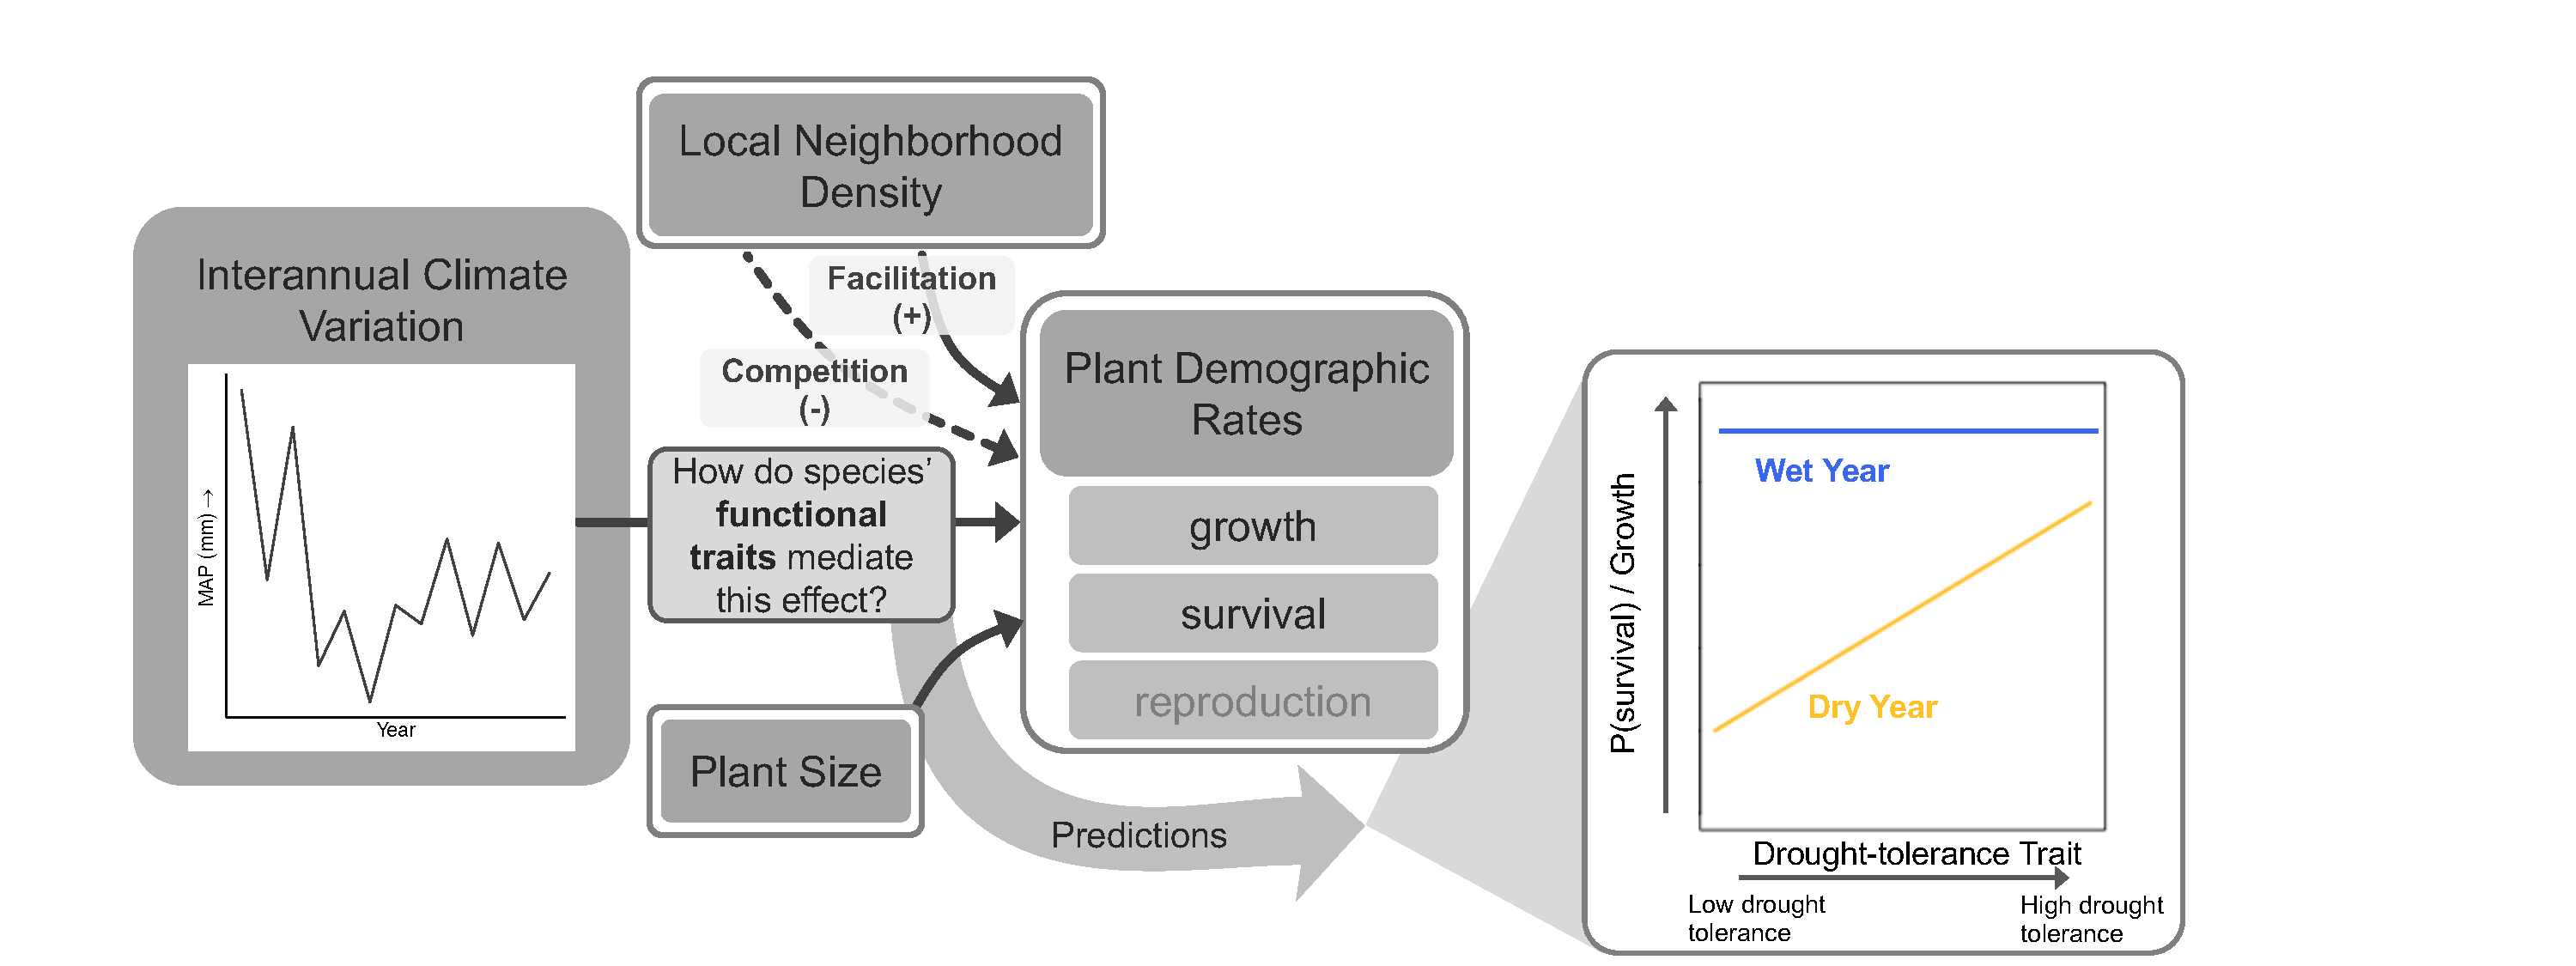
\includegraphics[width=1\textwidth]{CO_sgs_ConceptualFigure.pdf}
\caption{\internallinenumbers\small{
The demographic rates of growth, survival, and reproduction, are impacted by environmental variation, interactions with local neighbors, and plant size. We focus here on plant growth and survival due to a lack of information on recruitment rates. The impact of environmental variation on an organism's demographic rates is likely mediated by the functional traits of that organism. This is especially likely for traits that are related to environmental conditions that are most limiting or stress-inducing in a given habitat. In semiarid steppe, traits related to water use might be more important for plant growth and survival in very dry years, and relatively less important in years with high water availability. The figure on the right of this diagram shows how a trait related to drought-tolerance may mediate the effect of climate on growth and survival. Specifically, we predicted that water-use traits impact survival or growth rates in dry years, but are not important in wet years when a plant is not experiencing severe water stress. 
}
}
\label{fig:ConceptFig}
\end{figure}

\section{Methods}
\subsection{\textit{Demographic Data}} We monitored growth and survival for eight graminoid and eight forb species (Table \ref{TraitMeasurements}) in 24, 1-m$^2$ chart-quadrats from 1997 to 2010 at the Central Plains Experimental Research location (CPER) in Nunn, Colorado, USA (40.8$^o$N/110.8$^o$W). These quadrats were established as part of the Shortgrass Steppe Long Term Ecological Research project \cite{Chu2013}. This site is located at 1650 m elevation in the North American shortgrass steppe, which is dominated by \textit{Bouteloua gracilis} and \textit{Bouteloua dactyloides}. It receives an average of 340 mm of precipitation annually, and has a mean annual temperature of 8 $^o$C \cite{Chu2014}. Soils at the CPER are primarily Mollisols and Aridisols.

The chart-quadrat method used does not assign each individual a unique identifying number or tag, but does map each individual plant in a spatially explicit manner each year. Bunchgrasses, shrubs, and other plants with a sizeable basal area were mapped as polygons, while grasses and forbs with a small number of stems were mapped as points. Of the species included in this analysis, graminoids were measured as polygons, and forbs were measured as points, so each data type will be referenced as either "graminoids" or "forbs," respectively. Growth can only be extracted from this dataset for individuals measured as polygons, because size is not measured for points. We calculated growth as log(size$_{t+1}$/size$_t$) for each individual. 

We extracted growth and survival data from a digitized version of this map dataset using "tracking algorithms" in R statistical software \cite{Lauenroth2008, RCoreTeam2019}. These algorithms loop through the annual maps for a given quadrat, and assume that individuals of the same species growing in the same location in consecutive years are the same individual. In this way, the algorithms generate records of survival for all individuals, and records of growth or shrinkage for individuals measured as polygons. Individual plants can go dormant for up to several years, such that no above-ground material is visible. These tracking scripts allow for a user-defined period of dormancy, which we set to the conservative limit of one year. This means that if an individual is present in year one, absent from the maps in year two, but present in year three at the same coordinates as year one, this plant is considered to be the same individual. Allowing a longer dormancy period would likely lead to an over-estimate of survival, since new recruits in the same neighborhood as a con-specific individual in previous years would be more likely to be erroneously counted as that individual emerging from dormancy. We also allow a 'buffer' of 5 cm in observations of the same individual from year to year, which accounts for measurement error as well as true variation in re-sprouting location across years. The dataset of forb survival from 1997-2010 is dominated by \textit{Sphaeralcea coccinea}, which accounts for 78\% of the observations. To prevent \textit{S. coccinea} from skewing the results of the forb survival model, we randomly selected five individuals from each quadrat, and followed those individuals across the span of data collection. This reduces the size of the dataset, but makes the dataset more evenly distributed.

\subsection{\textit{Climate Data}} The standardized precipitation-evapotranspiration index (SPEI) is a metric of drought intensity that uses temperature and precipitation data to estimate evapotranspiration \shortcite{Vicente-Serrano2010}. To calculate SPEI for this analysis we used climate data from the Global SPEI database \cite{Vicente-Serrano2010}. We chose to use modeled climate data, as opposed to calculating SPEI by hand using observed climate data from the CPER site, since modeled data includes the data necessary to use the Penman-Monteith method of calculating potential evapotranspiration (PET). Only precipitation and temperature is available from the observed climate dataset, meaning it is only possible to calculate far inferior estimates of PET with this dataset. SPEI can be calculated over an interval as short as one month, or as long as 48 months. In this study, we used a four-month interval from May to June, which encapsulates the growing season for most species in the shortgrass steppe. 

\subsection{\textit{Trait Data}} We measured leaf and root functional traits for the graminoid, shrub, and forb species that comprise most of the diversity in the demographic dataset. Five to ten mature and healthy individuals of each target species were sampled for each trait measurement. A majority of the trait values used in this analysis were collected at the USDA-ARS CPER. Traits for several other species were measured at the USDA-ARS High Plains Grasslands Research Station (HPGRS) near Cheyenne, WY, a northern mixed-grass prairie within 35 miles of the CPER. Samples for trait measurement were collected at CPER and HPGRS between 2014 and 2018 \cite{Blumenthal2020}. In cases where trait values measured at CPER were not available, we used species-level trait values from samples at the University Pasture in Hays, KS (southern mixed-grass prairie), the USDA-ARS Ft. Keogh Livestock and Range Research Station in Miles City, MT (northern mixed-grass prairie), and the USDA-ARS US Sheep Experiment Station near Dubois, ID (sagebrush steppe). See Table \ref{TraitMeasurements} for a list of sampling locations for each species included in this analysis. 

We measured species-level average trait values for seven traits: specific leaf area (SLA; cm$^2$/g), leaf dry matter content (LDMC; g/g), turgor loss point (TLP; MPa), specific root length (SRL; g/m), average root diameter (RDiam; mm), root dry matter content (RDMC; g/g), and root tissue density (RTD; g/cm$^3$). SLA and LDMC were measured using standard methods \cite{Perez-Harguindeguy2013}. TLP was calculated from measurements of leaf osmotic potential made using a Vapro 5600 osmometer (Bartlett, Scoffoni, Ardy et al., \citeyearNP{Bartlett2012}). TLP was derived from osmotic potential using the following equations: graminoid leaf turgor loss point $= 0.944($leaf osmotic potential$)-0.611$ , forb leaf turgor loss point $= 0.80($leaf osmotic potential$)-0.845$ \cite{ Griffin-Nolan2019}. Below ground traits were measured for fine, absorptive root tissue (typically 1st-3rd order roots) \cite{McCormack2015}. Intact absorptive root branches were carefully extracted from soil monoliths, which were centered on the species of interest and sampled to 20 cm beneath the soil surface (Blumenthal et al., unpublished). Root length, average diameter, and root volume were measured using WinRhizo software (Regent Instruments, Inc., Ville de Québec, QC Canada). Further details of leaf trait sampling and measurement protocols can be found in \cite{Blumenthal2020}.

\subsection{\textit{Statistical Analysis}} We use a generalized linear mixed model (GLMM) framework to identify how the effect of trait values on growth and survival varies across a spectrum of drought intensity, as well as to assess the relative ability of each trait to predict these demographic rates. We created separate growth and survival models for each trait, since we are interested in the relative ability of each trait to predict drought tolerance along a gradient of SPEI. Both growth and survival models followed a similar covariate structure, shown here:
\begin{multline}
\label{surv_eq}
\textit{Response Variable} = \alpha + \gamma_{species}+ \delta_{quad} + \tau_{year} + ln(size_t(\beta_{species} + \beta_1)) +\\ trait\beta_2+ SPEI\beta_3 + nearEdge\beta_4 + neighborhoodDensity\beta_5 + (trait\times SPEI)\beta_6 + \epsilon 
\tag{\textbf{Equation 1}}
\end{multline}

To model survival, we used the lme4 package in R statistical software to fit GLMMs with a binomial error distribution and a logit link function \shortcite{RCoreTeam2019, Bates2015ParsimoniousModels}. Individual plant size, an important covariate, is only available for graminoids because forbs were mapped as points in this dataset. Because of this, we modeled graminoid and forb survival separately, and forb models do not contain a size covariate or a random slope for size. All survival models use a binary response variable indicating whether an individual survived (1) or died (0) in the next year (year$_\textit{t+1}$). Survival models included fixed terms for size (graminoids models only), SPEI, and neighborhood density in the current year (year$_\textit{t}$), a ‘nearEdge’ term that accounts for the potential impact of edge effects, trait value, and an interaction between trait and SPEI. These models also include random intercepts for species, quadrat, and year, and a random slope for plant size (graminoids models only) (Eqn. 1). Graminoid survival models using RTD and SRL did not include a random slope for plant size, since models including this term lead to singular model fit \shortcite{Bates2015}. 

 To model growth, we used the lme4 R package to fit linear mixed models using a Gaussian error distribution \shortcite{RCoreTeam2019, Bates2015ParsimoniousModels}. We measured growth as the natural logarithm of plant basal area in year$_\textit{t+1}$ as a function of basal area in year$_\textit{t}$ \shortcite{Dalgleish2011, Dahlgren2009LinkingHerb}. Growth models were only constructed for graminoids, since we did not have growth information for forbs. These models had an identical fixed and random covariate structure to graminoid survival models. All variables in all survival and growth models were scaled, and size$_{\textit{t}}$ and size$_{\textit{t+1}}$ were log-transformed and then scaled. In both model frameworks, the covariates of most interest are SPEI, trait, and the SPEI-by-trait interaction.
 
We included individual plant basal area (for graminoids) and conspecific local neighborhood density as fixed covariates in our models (Eqn. 1) to account for the effects of individual plant size \shortcite{Tredennick2018} and competition/facilitation on demographic rates (Fig. \ref{fig:ConceptFig}). Local neighborhood density was calculated for each individual in each year, and accounts for the effect of intra-specific competition or facilitation on demographic rates. For graminoids, the local neighborhood density is the total plant basal area within a 10 cm radius of the focal individual that is occupied by individuals of the same species (conspecifics). For forbs, this value is a sum of the total number of conspecific stems within a 10 cm local neighborhood radius of the focal individual. We calculated only intra-specific competition estimates, because the fact that forbs and graminoids were measured differently (forbs as a single point, graminoids as a polygon) made it difficult to produce a reasonable estimate of inter-specific competition. Additionally, it has been shown that inter-specific competition is typically weaker than intra-specific competition in dry grassland systems \cite{Chu2016, Laughlin2018}. We tested different neighborhood radii (5, 10, 15, and 20 cm) to determine which radius is the most appropriate to use in this ecological context by fitting four generalized linear mixed-effect models for the effect of a trait-by-environment interaction on survival (following the framework of Eqn. 1) while including a competition metric using a different radius in each model. We compared the size of the coefficient for the fixed effect of competition in each model, as well as the maximum likelihood of each model. The maximum likelihood indicated that both the 5 and 10 cm radii provided the best model fit, so we used a 10 cm local neighborhood radius. We also included a fixed effect, "nearEdge," which is a binary variable indicating whether an individual was growing within 5 cm of the quadrat edge. This covariate accounts for the higher probability of ’missing’ an edge individual during mapping, as well as potential under-estimation of local neighborhood density or individual size due to proximity to the quadrat edge.

All models included a random intercept for quadrat (1\textbar quad) to account for non-independence of observations within the same quadrat, and a random intercept for year (1\textbar year) to account for non-independence of samples observed in the same year. Because data on individual size was available for graminoids, we included a random slope for size associated with a random intercept for species (size$_\textit{t}$\textbar species), which accounts for the fact that larger individuals of a given species have a higher growth and survival probability than small individuals, but also allows for variation in response for each species. 

We used AIC to determine the best random effect structure for each trait model by comparing the F-statistics of models with all possible random effect structures. We then used an analogous process to determine the best fixed effect structure \cite{Bolker2009}. We used the size and significance of the trait-by-SPEI interaction coefficient to rank traits by their respective ability to predict drought tolerance. Because data for each trait was not available for all species, each model had a slightly different sample size, making it impossible to use AIC to compare fit across models. Instead, we used AIC to compare each model to a model of the same structure, but without the trait and trait-by-environment interaction coefficients (recorded as $\Delta$ AIC in Tables \ref{ModResults}, \ref{growth_ModResults}, and \ref{ForbSurv_ModResults}). This comparison indicates the extent to which traits improve the models. The larger the decrease in AIC in the trait model relative to the no-trait model, the more support for the ability of that trait to predict survival or growth in response to drought. Positive $\Delta$ AIC values indicate that including a trait improved model fit, while negative $\Delta$ AIC values indicate that including a trait did not improve model fit. We also used likelihood ratio tests as an additional method to determine the extent to which models including traits were better than models without traits.

\section{Results}
\subsection{\textit{Graminoid Survival}} 
We detected significant positive main effects of individual plant size and significant negative main effects of local neighborhood conspecific density on survival probability across all trait models (Table \ref{ModResults}; Fig. \ref{fig:Effects_Survival}). In other words, larger plants were more likely to survive than smaller plants of the same species, and individuals that share their immediate local environment with more individuals of the same species were less likely to survive. There was a consistently negative main effect of SPEI on survival probability, although this effect was only significant in the model using root diameter (RDiam). This negative coefficient suggests that plants had a higher survival probability when less water was available, which contradicts our predictions. In most cases, except for the positive effect of RTD, the main effects of traits by themselves on survival were not significant, and their effects were only manifested through interactions with SPEI. Variation in the modeled fixed and random effects explained between 33 and 67\% of the variation in survival rates (Table \ref{ModResults}).

Models of survival for graminoids indicated that every trait except for SRL interacted with SPEI to impact survival (Table \ref{ModResults}). The traits with the largest interaction coefficients were LDMC ($\beta _6=$-0.26, \textit{P} $<$0.01), RDMC ($\beta _6=$-0.21, \textit{P} $<$0.01), and TLP ($\beta _6=$0.15, \textit{P} $<$0.01)(Table \ref{ModResults}; Fig. \ref{fig:PredsObs}: \textbf{A}, \textbf{D}, \textbf{G}, \textbf{J} and \textbf{M}). Species with lower leaf TLP and species with higher LDMC and RDMC were more likely to survive in dry years than wet years. The opposite was true of species with higher TLP and lower LDMC and RDMC. $\Delta$ AIC values and likelihood ratio test statistics indicated that LDMC, RDMC, TLP, and RDiam were the traits that best predicted how survival probability changed across a gradient of SPEI (Table \ref{ModResults}).

\subsection{\textit{Graminoid Growth}} 
We detected significant positive main effects of individual plant size in the current year on size in the next year across all trait models (\textit{P} $<0.01$)(Table \ref{growth_ModResults}; Fig. \ref{fig:Effects_Growth}). Even though this effect is positive, it is never above zero. When plants are small, they are likely to become larger in the following year. However, when they exceed a moderate size in the current year, they are likely to shrink in the following year. This is shown in Fig. \ref{fig:Effects_Growth}: \textbf{B} and \textbf{C}, where at a smaller value of size$_{\textit{t}}$, lines showing the average relationship between size$_{\textit{t}}$ and size$_{\textit{t+1}}$ are above the 1:1 dashed line, while at larger sizes of size$_{\textit{t}}$, the fitted lines are below the dashed line. Across all models of plant growth, there was a significant negative main effect of local neighborhood conspecific density (\textit{P} $<0.01$)(Table \ref{growth_ModResults}).

Models of graminoid growth did not identify any significant interactions between trait and SPEI (Table \ref{growth_ModResults}, Fig. \ref{fig:PredsObs}: \textbf{B}, \textbf{E}, \textbf{H}, \textbf{K}, \textbf{N}). Species with trait values across the spectrum of measured traits were more likely to become larger in the next year when SPEI was higher, although this relationship was only statistically significant in models using TLP ($\beta _2=$0.12, \textit{P} $<$0.05), LDMC ($\beta _2=$0.13, \textit{P} $<$0.05), SLA ($\beta _2=$0.12, \textit{P} $<$0.05), RDMC ($\beta _2=$0/12, \textit{P} $<$0.05), and RDiam ($\beta _2=$0.12, \textit{P} $<$0.05). Species with low TLP ($\beta _2=$-0.17, \textit{P} $<$0.05) and low RTD ($\beta _2=$-0.20, \textit{P} $<$0.05) were significantly more likely to grow larger in the next year. Negative $\Delta$ AIC values for all models indicated that including a trait and trait-by-SPEI interaction made model fit worse (Table \ref{growth_ModResults}). Additionally, likelihood ratio tests did not identify any significant differences between growth models with and without traits (Table \ref{growth_ModResults}). These growth models including traits and trait-by-SPEI interactions explained 16-53\% of the variation in growth rates (Table \ref{growth_ModResults}). 

\subsection{\textit{Forb Survival}} 
There were no effects of local neighborhood conspecific density, SPEI, or traits on forb survival (Table \ref{ForbSurv_ModResults}). Marginal R$^2$ values were much smaller for forb models than graminoid models (all $<0.1$); conditional R$^2$ values ranged from 0.49 to 0.64 (Table \ref{ForbSurv_ModResults}). However, models of plant survival for forbs indicated that survival is affected by a significant interaction between SPEI and LDMC ($\beta_6=$-0.38, \textit{P} $<$0.01), RDMC ($\beta _6=$-0.31, \textit{P} $<$0.05), SLA ($\beta _6=$0.57, \textit{P} $<$0.05), and RTD ($\beta _6=$-0.27, \textit{P} $<$0.05) (Table \ref{ForbSurv_ModResults}), (Fig. \ref{fig:PredsObs}: \textbf{C}, \textbf{F}, \textbf{I}, \textbf{L} and \textbf{O}). In dry years, survival was higher for species with lower leaf TLP and species with high LDMC and RDMC. In wet years, survival was higher for species with high TLP and low LDMC and RDMC; however, species with low TLP and high LDMC and RDMC had lower survival probability in wet years than in dry years. These patterns are consistent with those observed for graminoid survival. The interaction between SLA and SPEI for forb survival, however, was different than the pattern observed in graminoids. Low SLA species had high survival in dry years and low survival in wet years, where a strongly opposite pattern occurred for high SLA species. The uncertainty in these estimates was much larger for forb survival models than graminoid models, as illustrated by the 95\% confidence intervals (Fig. \ref{fig:PredsObs}; Fig. \ref{fig:GramSurv_all}). $\Delta$ AIC values were highest for models with LDMC, RDMC, and SLA, which indicated that including coefficients for trait and trait-by-SPEI interactions for those traits improved our ability to predict how survival probability changes with variation in SPEI (Table \ref{ForbSurv_ModResults}). Likelihood ratio tests only identified a significant improvement of trait models over no-trait models for models using LDMC (Table \ref{ForbSurv_ModResults}). 


\begin{table}[h] \centering 
 \caption{\internallinenumbersGraminoid Survival Model Coefficients} 
 \label{ModResults} 
 \resizebox{\textwidth}{!}{%
\begin{tabular}{lccccccc} 
\\[-1.8ex]\hline 
\hline \\[-1.8ex] 
 & \multicolumn{7}{c}{\textit{Trait Model}} \\ 
\cline{2-8} 
\\
\\[-1.8ex] & TLP & LDMC & SLA & RDMC & RTD & SRL & RDiam\\ 
\hline \\[-1.8ex] 
 \rowcolor[gray]{.95}size_t & 1.03$^{***}$ & 0.94$^{***}$ & 0.96$^{***}$ & 0.78$^{***}$ & 1.19$^{***}$ & 1.20$^{***}$ & 0.86$^{***}$ \\
 neighbors & $-$0.61$^{***}$ & $-$0.62$^{***}$ & $-$0.60$^{***}$ & $-$0.61$^{***}$ & $-$0.43$^{***}$ & $-$0.43$^{***}$ & $-$0.59$^{***}$ \\
\rowcolor[gray]{.95}nearEdge & 0.004 & $-$0.001 & 0.01 & $-$0.003 & 0.08$^{*}$ & 0.08$^{*}$ & 0.02 \\ 
 \textbf{SPEI:trait} & 0.16$^{***}$ & $-$0.26$^{***}$ & $-$0.08$^{***}$ & $-$0.21$^{***}$ & 0.01 & $-$0.05$^{**}$ & $-$0.15$^{***}$ \\ 
 \rowcolor[gray]{.95}SPEI & $-$0.08 & $-$0.09 & $-$0.07 & $-$0.11 & $-$0.23$^{*}$ & $-$0.23$^{*}$ & $-$0.19$^{**}$ \\
 \textbf{trait} & $-$0.13$^{**}$ & 0.26$^{**}$ & $-$0.07 & $-$0.02 & 0.36$^{***}$ & 0.14 & $-$0.04 \\ 
 \rowcolor[gray]{.95}Intercept & $-$2.34$^{***}$ & $-$2.13$^{***}$ & $-$2.32$^{***}$ & $-$2.02$^{***}$ & $-$2.17$^{***}$ & $-$2.00$^{***}$ & $-$2.17$^{***}$ \\  
 \hline \\[-1.8ex] 
 $\tau_{00}$ & 0.13$_{quad}$ & 0.12$_{quad}$ & 0.13$_{quad}$ & 0.13$_{quad}$ & 0.11$_{quad}$ & 0.11$_{quad}$ & 0.12$_{quad}$ \\
 & 0.11$_{year}$ & 0.12$_{year}$ & 0.09$_{year}$ & 0.08$_{year}$ & 0.14$_{year}$ & 0.14$_{year}$ & 0.08$_{year}$ \\
 & 1.58$_{spp.}$ & 1.70$_{spp.}$ & 1.27$_{spp.}$ & 0.48$_{spp.}$ & 0.06$_{spp.}$ & 0.40$_{spp.}$ & 0.58$_{spp.}$\\
 \rowcolor[gray]{.95}$\tau_{11}$ & 0.38$_{size_t*spp}$ & 0.30$_{size_t*spp}$ & 0.37$_{size_t*spp}$ &
 0.15$_{size_t*spp}$ & & & 0.17$_{size_t*spp}$ \\
 $\rho_{01}$ & $-$0.99$_{spp.}$ & $-$0.97$_{spp.}$ & $-$0.96$_{spp.}$ & $-$0.85$_{spp.}$ & & & $-$0.88$_{spp.}$ \\
\hline \\[-1.8ex] 
\rowcolor[gray]{.95} Residual Variance & 3.29 & 3.29 & 3.29 & 3.29 & 3.29 & 3.29 & 3.29\\
n & 18,750 & 18,827 & 18,827 & 18,474 & 16,618 & 16,618 & 17,190\\ 
\rowcolor[gray]{.95} Marg./Cond. $R^2$ & 0.43/0.65	& 0.41/0.62 &	0.38/0.63 & 0.33/0.50 & 0.61/0.64 &	0.60/0.67 & 0.38/0.55 \\
AIC  & 14,722.07 & 14,749.38 & 14,861.92 & 14,774.85 & 13,344.33 & 13,346.40 & 13,502.53 \\ 
\hline 
\rowcolor[gray]{.95}$\Delta$ AIC$^\dagger$ & 55.79 & 123.18 & 10.64 & 87.60 & 5.06 & 2.99 & 46.13 \\
LRT:  $\chi^2$(df)$^{\dagger\dagger}$ & 59.8(2)$^{***}$ & 127.2(2)$^{***}$ & 14.6(2)$^{***}$ & 91.6(2)$^{***}$ & 9.1(2)$^{**}$ & 7.0(2)$^{**}$ & 50.1(2)$^{***}$\\
\hline 
\hline \\[-1.8ex] 
\textit{Note:} & \multicolumn{7}{r}{$^{*}$ \textit{P} $<$0.1; $^{**}$ \textit{P} $<$0.05; $^{***}$ \textit{P} $<$0.01}\\
\multicolumn{8}{l}{$\tau_{00}$ = Rand. Intercept Variance; $\tau_{01}$=Rand. Slope Variance; $\rho_{01}$=Correlation of Rand. Slope \& Intercept}\\ 
\multicolumn{8}{l}{$^\dagger$ = compares the AIC of a model with trait and trait:envi interaction as fixed effects to a model without}\\
\multicolumn{8}{l}{trait and trait:envi effects. This serves as a relative metric of the predictive power of a given trait.}\\
\multicolumn{8}{l}{$^{\dagger\dagger}$ = Results from a likelihood ratio test comparing models with and without trait and trait:envi effects.}\\
\multicolumn{8}{l}{Significant $\chi^2$ values indicate that the model with trait and a trait:envi terms provides a significantly }\\
\multicolumn{8}{l}{better fit to the data than the model without those terms. Insignificant $\chi^2$ values indicate that there is no}\\
\multicolumn{8}{l}{significant difference between models.}
\end{tabular}} 
\end{table} 


\begin{table}[h] \centering 
 \caption{\internallinenumbersGraminoid Growth Model Coefficients} 
 \label{growth_ModResults} 
 \resizebox{\textwidth}{!}{
\begin{tabular}{lccccccc} 
\\[-1.8ex]\hline 
\hline \\[-1.8ex] 
 & \multicolumn{7}{c}{\textit{Trait Model}} \\ 
\cline{2-8} \\ 
\\[-1.8ex] & TLP & LDMC & SLA & RDMC & RTD & SRL & RDiam\\ 
\hline \\[-1.8ex] 
 \rowcolor[gray]{.95}size$_{t}$ & 0.48$^{***}$ & 0.51$^{***}$ & 0.51$^{***}$ & 0.51$^{***}$ & 0.56$^{***}$ & 0.56$^{***}$ & 0.48$^{***}$ \\
 neighbors & $-$0.12$^{***}$ & $-$0.12$^{***}$ & $-$0.12$^{***}$ & $-$0.12$^{***}$ & $-$0.13$^{***}$ & $-$0.13$^{***}$ & $-$0.13$^{***}$ \\ 
 \rowcolor[gray]{.95}nearEdge & $-$0.003 & $-$0.004 & $-$0.004 & $-$0.004 & $-$0.03 & $-$0.03 & $-$0.02 \\ 
 \textbf{SPEI:trait} & 0.01 & $-$0.02 & $-$0.004 & $-$0.01 & 0.01 & 0.003 & $-$0.02 \\ 
\rowcolor[gray]{.95} SPEI\_s & 0.12$^{**}$ & 0.13$^{**}$ & 0.12$^{**}$ & 0.12$^{**}$ & 0.12$^{*}$ & 0.12$^{*}$ & 0.12$^{**}$ \\ 
 \textbf{trait} & $-$0.19$^{**}$ & 0.13 & 0.05 & 0.05 & $-$0.20$^{**}$ & $-$0.09 & 0.02 \\ 
 \rowcolor[gray]{.95} Intercept & 1.47$^{***}$ & 1.44$^{***}$ & 1.27$^{***}$ & 1.33$^{***}$ & 1.09$^{***}$ & 1.01$^{***}$ & 1.32$^{***}$ \\ 
 \hline \\[-1.8ex] 
 $\tau_{00}$ & 0.02$_{quad}$ & 0.02$_{quad}$ & 0.02$_{quad}$ & 0.02$_{quad}$ & 0.02$_{quad}$ & 0.02$_{quad}$ & 0.02$_{quad}$ \\
 & 0.03$_{year}$ & 0.03$_{year}$ & 0.03$_{year}$ & 0.03$_{year}$ & 0.04$_{year}$ & 0.04$_{year}$ & 0.04$_{year}$ \\
 & 0.82$_{spp.}$ & 0.60$_{spp.}$ & 0.53$_{spp.}$ & 0.52$_{spp.}$ & 0.34$_{spp.}$ & 0.49$_{spp.}$ & 0.76$_{spp.}$\\
 \rowcolor[gray]{.95}$\tau_{11}$ & 0.07 $_{size_t*spp}$ & 0.06$_{size_t*spp}$ & 0.06$_{size_t*spp}$ &
 0.06$_{size_t*spp}$ & 0.08$_{size_t*spp}$ & 0.07$_{size_t*spp}$ & 0.09$_{size_t*spp}$ \\
 $\rho_{01}$ & $-$0.90$_{spp.}$ & $-$0.86$_{spp.}$ & $-$0.81$_{spp.}$ & $-$ 0.78$_{spp.}$ & $-$0.74$_{spp.}$ & $-$0.48$_{spp.}$ & $-$0.76$_{spp.}$ \\
\hline \\[-1.8ex] 
\rowcolor[gray]{.95} Residual Variance & 1.44 & 1.44 & 1.44 & 1.44 & 1.45 & 1.45 & 1.45 \\
n & 9,480 & 9,497 & 9,497 & 9,497 & 8,802 & 8,802 & 9,018 \\ 
\rowcolor[gray]{.95} Marg./Cond. R$^2$ & 0.21/0.38 & 0.23/0.40	& 0.20/0.40 & 0.20/0.41	& 0.24/0.49 & 0.19/0.53 & 0.16/0.44\\
AIC & 30,536.16 & 30,597.42 & 30,600.18 & 30,599.27 & 28,430.58 & 28,433.69 & 29,107.74 \\ 
\hline 
\rowcolor[gray]{.95}$\Delta$ AIC$^\dagger$ & $-$10.76 & $-$10.40 & $-$13.16 & $-$12.25 & $-$9.55 & $-$12.66 & $-$12.39 \\
LRT:  $\chi^2$(df)$^{\dagger\dagger}$ &
2.8(2) & 2.6(2) & 0.6(2) & 0.5(2) & 4.4(2) & .0.8(2) & 0.7(2)\\
\hline 
\hline \\[-1.8ex] 
\textit{Note:} & \multicolumn{7}{r}{$^{*}$ \textit{P} $<$0.1; $^{**}$ \textit{P} $<$0.05; $^{***}$ \textit{P} $<$0.01}\\
\multicolumn{8}{l}{$\tau_{00}$ = Rand. Intercept Variance; $\tau_{01}$=Rand. Slope Variance; $\rho_{01}$=Correlation of Rand. Slope \& Intercept}\\
\multicolumn{8}{l}{$^\dagger$ = compares the AIC of a model with trait and trait:envi interaction as fixed effects to a model without}\\
\multicolumn{8}{l}{trait and trait:envi effects. This serves as a relative metric of the predictive power of a given trait.}\\
\multicolumn{8}{l}{$^{\dagger\dagger}$ = Results from a likelihood ratio test comparing models with and without trait and trait:envi effects.}\\
\multicolumn{8}{l}{Significant $\chi^2$ values indicate that the model with trait and a trait:envi terms provides a significantly }\\
\multicolumn{8}{l}{better fit to the data than the model without those terms. Insignificant $\chi^2$ values indicate that there is no}\\
\multicolumn{8}{l}{significant difference between models.}
\end{tabular}} 
\end{table} 


\begin{table}[h] \centering 
 \caption{\internallinenumbers Forb Survival Model Coefficients} 
 \label{ForbSurv_ModResults} 
 \resizebox{\textwidth}{!}{%
\begin{tabular}{lccccccc} 
\\[-1.8ex]\hline 
\hline \\[-1.8ex] 
 & \multicolumn{7}{c}{\textit{Trait Model}} \\ 
\cline{2-8} 
\\
\\[-1.8ex] & TLP & LDMC & SLA & RDMC & RTD & SRL & RDiam\\ 
\hline \\[-1.8ex] 
 neighbors & $-$0.17 & $-$0.24 & $-$0.24 & $-$0.23 & $-$0.15 & $-$0.17 & $-$0.16 \\ 
 \rowcolor[gray]{.95}nearEdge & 0.05 & $-$0.01 & $-$0.08 & $-$0.02 & 0.16 & 0.11 & 0.05 \\ 
 \textbf{SPEI:trait} & 0.13 & -0.38$^{***}$ & 0.57$^{**}$ & -0.31$^{**}$ & -0.27$^{**}$ & 0.20 & 0.02\\ 
 \rowcolor[gray]{.95}SPEI & 0.22 & 0.29 & 0.37$^{*}$ & 0.20 & 0.26 & 0.26 & 0.19 \\
 \textbf{trait} & $-$0.60 & $-$0.19 & 0.22 & $-$0.39 & 0.14 & 0.07 & 0.08 \\
 \rowcolor[gray]{.95}Intercept & $-$1.11 & $-$1.80$^{**}$ & $-$1.64$^{**}$ & $-$2.01$^{***}$ & $-$1.09 & $-$2.02$^{*}$ & $-$1.67$^{**}$ \\ 
\hline \\[-1.8ex] 
 $\tau_{00}$ & 0.28$_{quad}$ & 0.26$_{quad}$ & 0.30$_{quad}$ & 0.27$_{quad}$ & 0.38$_{quad}$ & 0.40$_{quad}$ & 0.29$_{quad}$ \\
 & 0.35$_{year}$ & 0.28$_{year}$ & 0.30$_{year}$ & 0.31$_{year}$ & 0.43$_{year}$ & 0.50$_{year}$ & 0.41$_{year}$ \\
 & 2.30$_{spp.}$ & 2.33$_{spp.}$ & 2.64$_{spp.}$ & 2.68$_{spp.}$ & 2.33$_{spp.}$ & 4.84$_{spp.}$ & 3.06$_{spp.}$\\
\hline \\[-1.8ex] 
\rowcolor[gray]{.95} Residual Variance & 3.29 & 3.29 & 3.29 & 3.29 & 3.29 & 3.29 & 3.29\\
n & 456 & 499 & 499 & 499 & 388 & 414 & 456 \\ 
\rowcolor[gray]{.95} Marg./Cond. $R^2$ & 0.06/0.50 & 0.04/0.49 & 0.03/0.51 &	0.04/0.51 & 0.02/0.50 &	0.01/0.64 &	0.01/0.54\\
AIC & 567.28 & 583.88 & 587.13 & 587.47 & 496.77 & 502.25 & 568.82 \\ 
\hline 
\rowcolor[gray]{.95}$\Delta$ AIC$^\dagger$ & $-$2.37 & 4.63 & 1.39 & 1.05 & $-$0.90 & $-$2.87 & $-$3.91 \\
LRT:  $\chi^2$(df)$^{\dagger\dagger}$ &
1.6(2) & 8.6(2)$^{**}$ & 5.3(2)$^{*}$ & 5.0(2)$^{*}$ & 3.1(2) & 1.1(2) & 0.1(2)\\
\hline 
\hline \\[-1.8ex] 
\textit{Note:} & \multicolumn{7}{r}{$^{*}$ \textit{P}$<$0.1; $^{**}$ \textit{P}$<$0.05; $^{***}$ \textit{P}$<$0.01} \\ 
\multicolumn{8}{l}{$\tau_{00}$ = Rand. Intercept Variance}\\
\multicolumn{8}{l}{$^\dagger$ = compares the AIC of a model with trait and trait:envi interaction as fixed effects to a model without}\\
\multicolumn{8}{l}{trait and trait:envi effects. This serves as a relative metric of the predictive power of a given trait.}\\
\multicolumn{8}{l}{$^{\dagger\dagger}$ = Results from a likelihood ratio test comparing models with and without trait and trait:envi effects.}\\
\multicolumn{8}{l}{Significant $\chi^2$ values indicate that the model with trait and a trait:envi terms provides a significantly }\\
\multicolumn{8}{l}{better fit to the data than the model without those terms. Insignificant $\chi^2$ values indicate that there is no}\\
\multicolumn{8}{l}{significant difference between models.}
\end{tabular} }
\end{table} 

\begin{figure}[h]
  \centering
  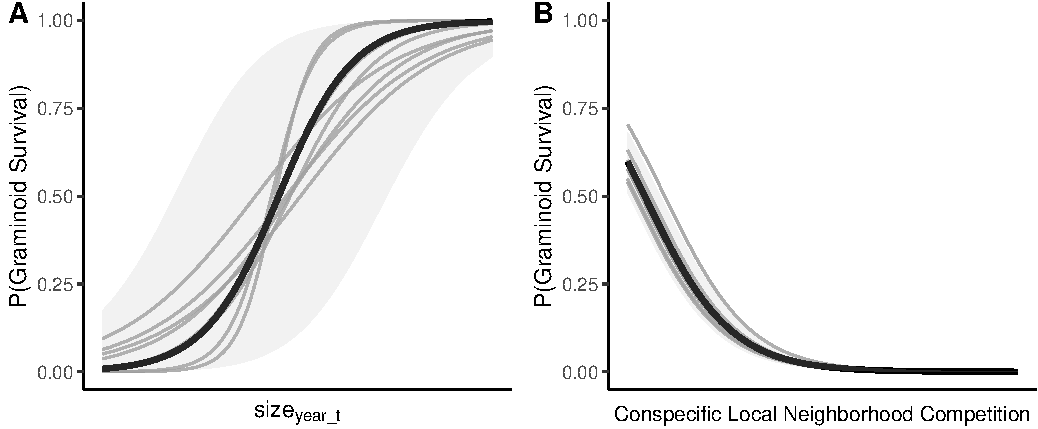
\includegraphics[width=.8\textwidth]{survEffectPlots-1.pdf}
  \caption{\internallinenumbers The effect of local neighborhood density (\textbf{A}) and size in year$_\textit{t}$ (\textbf{B}) on graminoid survival in models using LDMC as the trait predictor. Across all graminoid species, higher crowding of an individual’s local neighborhood (10 cm radius) with individuals of the same species corresponds with lower survival probability (\textbf{A}), and larger individuals are more likely to survive to the next year than smaller individuals of the same species (\textbf{B}). Dark lines indicate the overall effect of each covariate on survival. The 95\% confidence interval for the overall effect of conspecific local neighborhood competition is shown in light greys. Colored lines incorporate random species effects to indicate the effect of competition or size for each species.}
  \label{fig:Effects_Survival}
\end{figure}

\begin{figure}[h]
  \centering
  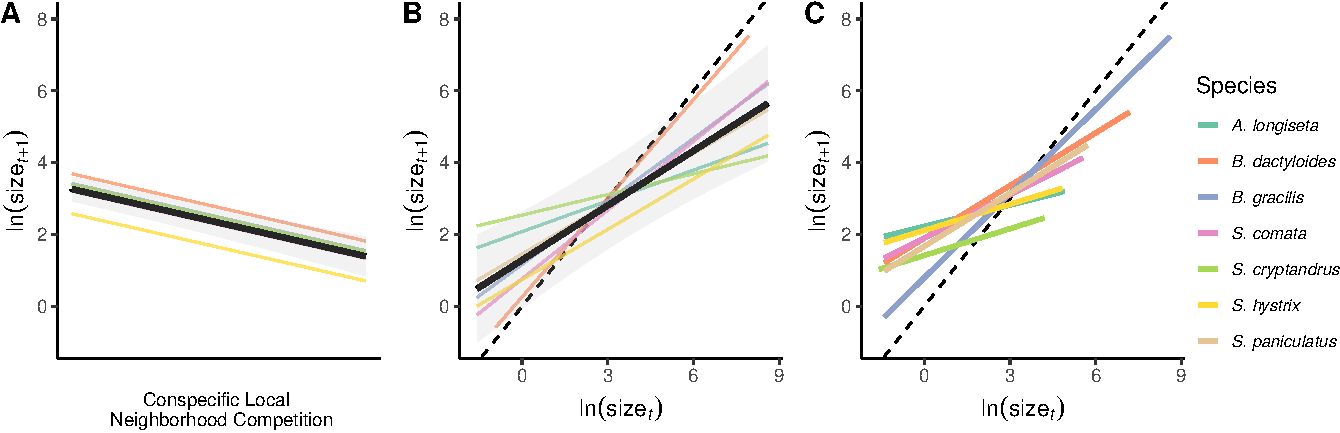
\includegraphics[width=1\textwidth]{figures/growthEffectPlots-1.pdf}
  \caption{\internallinenumbers(\textbf{A}) shows the effect of local neighborhood density on graminoid size in year$_\textit{t+1}$ in models using TLP as the trait predictor. Across all graminoid species, higher crowding of an individual’s local neighborhood (10 cm radius) with individuals of the same species corresponds to smaller size$_\textit{t+1}$. (\textbf{B}) shows the \textit{modeled} effect of size in year$_\textit{t}$ on size in year$_\textit{t+1}$ in models using TLP as the trait predictor. As size$_\textit{t}$ increases, a plant is more likely to become larger in year$_\textit{t+1}$ until it reaches a mid-point in size$_\textit{t}$, at which it becomes less likely to grow larger in year$_\textit{t+1}$. (\textbf{C}) In the \textit{raw data}, there is a positive linear relationship between ln(size$_\textit{t}$) and ln(size$_{t+1}$) for each of the eight graminoid species included in the growth analysis, although there is a size above which plants are more likely to shrink than grow in year$_\textit{t}$. The dashed lines in (\textbf{B}) and (\textbf{C}) indicate a 1:1 relationship between ln(size$_\textit{t}$) and ln(size$_\textit{t+1}$). Lines above the dashed line indicate growth, while lines below the dashed line indicate shrinkage. Dark lines indicate the overall effect of each covariate on survival The 95\% confidence interval for the overall effect of conspecific local neighborhood competition is shown in light grey. Colored lines incorporate random species effects to indicate the effects of competition or size$_{t}$ on size$_{t+1}$ for each species. 
  }
  \label{fig:Effects_Growth}
\end{figure}

\begin{figure}
\captionsetup{labelformat=empty}
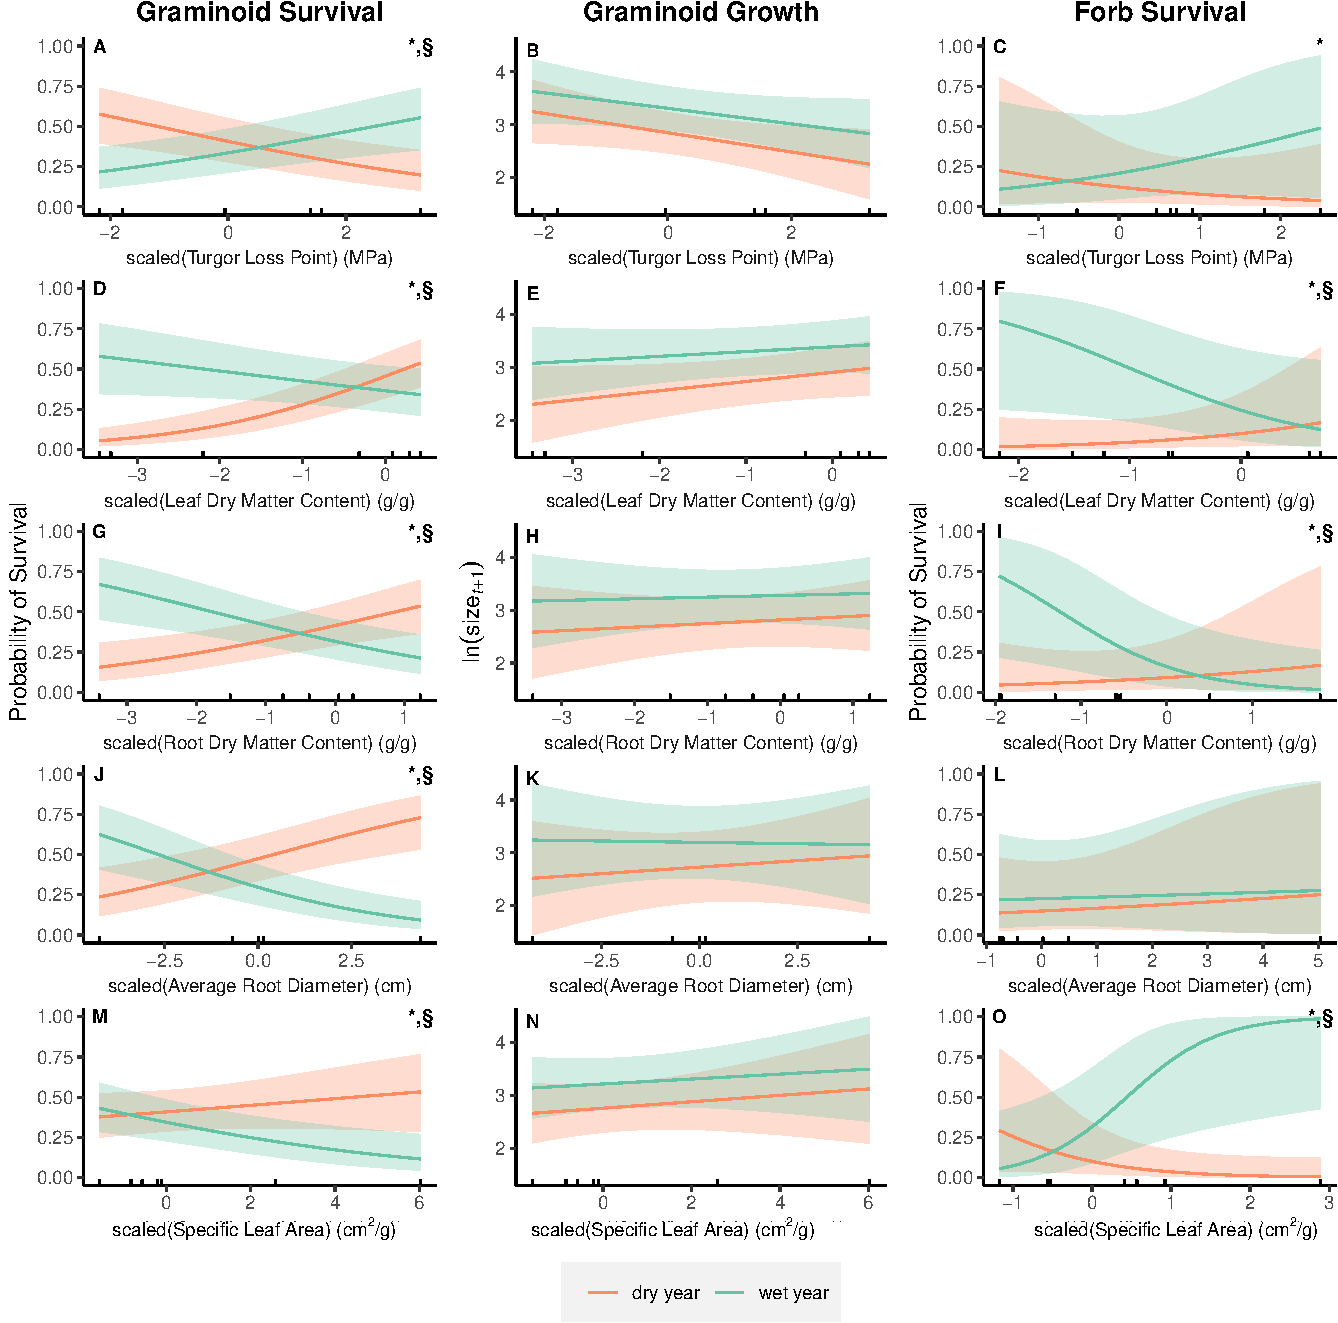
\includegraphics[width=1\textwidth]{mainObservationsFig-1.pdf}
\caption{}
\label{fig:PredsObs}
\end{figure}
\clearpage

\begin{figure}[h]
  %\captionsetup{labelformat=adja-page}
  \ContinuedFloat
  \caption{\internallinenumbers
(\textbf{A}) Graminoid species are more likely to survive in dry years (low SPEI, orange line) if they have a low TLP than if they have high TLP, while species with a high TLP are slightly more likely to survive in wet years (high SPEI, green line). 
(\textbf{D}) A similar trend in graminoid survival probability is predicted by the model that includes LDMC. 
(\textbf{G}) A similar trend to LDMC exists for graminoid survival probability as predicted by the interaction between RDMC and SPEI. 
(\textbf{J}) There is a significant interaction between RDiam and SPEI, but including RDiam does not greatly improve model fit in comparison to a model without trait values.
(\textbf{M}) SLA does interact with SPEI to affect graminoid survival, but does not greatly improve model fit in comparison to a model without trait values. 
(\textbf{B, E, H, K, N}) There is not a significant interaction between the effects of any trait and SPEI on size$_\textit{t+1}$. However, Low TLP graminoid species are larger in year$_\textit{t+1}$ than high TLP species both in wet years (high SPEI, green line) and in dry years (low SPEI, orange line). Horizontal dashed lines in (\textbf{B, E, H, K}, \textbf{N}) indicate the average plant size in year$_\textit{t}$. 
(\textbf{C}, \textbf{F}, \textbf{I}, \textbf{L}, \textbf{O}) Trends for forb survival were similar to those observed for graminoids, although the model fit is weaker and the interaction between trait and environment is less significant for each trait.
Black vertical bars along the x-axis (rug plots) indicate the trait values of the species included in each analysis. Survival probabilities and ln(size$_\textit{t+1}$) for 'wet years' and 'dry years' are calculated for the 97.5$^{th}$ and 2.5$^{th}$ quantiles of the distribution of SPEI values. \\
* indicates that this trait-by-SPEI interaction is significant (\textit{P} $<$ 0.05)\\
§ indicates that $\Delta$ AIC for this model is positive
}
 \label{fig:test}
\end{figure}
\section{Discussion}
The demographic processes of growth, survival, and reproduction are the underlying drivers of plant population and community dynamics, and the impact of climate change on vegetation will emerge via its effects on these demographic rates. However, the effects of climate change on demographic rates are mediated by functional traits, which determine the plant’s physiological response. By defining how functional traits mediate abiotic effects on demographic rates, we may be able to predict how other species will respond to environmental change. This approach is substantially less data-intensive than traditional species-based methods, and could be applied at broad scales across multiple systems. 

We determined how morphological and physiological functional traits mediated the effect of drought on perennial growth and survival in a shortgrass steppe ecosystem, using 15 years of demographic data, species-level trait measurements, and measurements of interannual climate variation. We found that (1) traits are more important for predicting survival than growth across a gradient of SPEI in this ecosystem, (2) leaf TLP is an important predictor of survival probability and growth in this semiarid grassland ecosystem, (3) RDMC and LDMC are more tightly related than TLP to survival in both graminoids and forbs, and (4) survival is not uniformly higher for all species in wet years.

Wilcox et al. (2020) found that the population-level response to precipitation in shortgrass steppe species (as measured by annual changes in percent-cover and ANPP) could be predicted by species-level values of TLP, LDMC, and SLA, as well as leaf N and P. The net effects of traits on the demographic parameters of survival generally agree with the relationships identified by Wilcox, et al. (2020). Species with trait values that we predicted to be drought tolerant (low TLP, high LDMC and RDMC) were more likely to survive in dry years and less likely to survive in wet years than their counterparts at the other end of the trait spectrum (Fig. \ref{fig:PredsObs}: \textbf{A, D, G, J} and \textbf{M}).

Species with low TLP and high leaf and root DMC also had relatively high growth in comparison to their high TLP and low DMC counterparts, yet these associates were not sensitive to SPEI (Fig. \ref{fig:PredsObs}: \textbf{B, E, H, K} and \textbf{N}). Species with trait values considered to be more drought tolerant grew larger regardless of drought intensity. These results are inconsistent with the pattern identified in Wilcox, et al. (2020), which could suggest that growth has relatively low importance for population-level responses to drought, and that survival could be the limiting demographic process driving plant population responses to lack of water in this ecosystem. Once a plant survives to the the following year, its size in that year is not significantly impacted by water availability. However, it is possible that increased measurement error for growth values undermined our ability to detect a significant interactive effect of drought and traits on growth. There is substantial room for error both when translating a basal area outline from a 1 m$^2$ quadrat to a hand-held datasheet, and when converting these analog maps to digitized shapefiles. This source of error is compounded by the human error that inevitably results when many different people collect data over many years. As such, the question of whether survival is more important than growth for population growth rate in this system requires further study. Regardless of potential error, these analyses indicate that the probability that a perennial grass will survive to the next year depends on both that grass’s trait values, and the SPEI of the current year. Whereas that grass's size in the next year is dictated by its trait values in the same way regardless of whether the current year is wet or dry. This result highlights the importance of considering multiple vital rates, since studies that only consider one vital rate have the potential to draw inaccurate conclusions about how traits mediate abiotic impacts on fitness. To generate a complete picture of how traits determine plant fitness in different environments, it will be necessary to either explicitly consider their effects on growth, survival and reproduction, or quantify fitness by measuring intrinsic population growth rates \cite{Laughlin2020TheFitness}.

Leaf TLP, a physiological trait that quantifies osmotic resistance to wilting, is a good predictor of plant survival and growth in the shortgrass steppe ecosystem where water availability is highly variable and limits plant growth (Fig. \ref{fig:PredsObs}) \cite{Lauenroth1992Long-TermSteppe}. TLP has long been used as an indicator of physiological drought tolerance, and has been linked to drought tolerance in tropical tree species (Bartlett, Scoffoni, Ardy et al., \citeyearNP{Bartlett2012}). However, there is mixed evidence for it’s utility as a predictor of drought tolerance in grasslands. Leaf TLP has been linked to precipitation sensitivity in North American grasslands \cite{Griffin-Nolan2019, Blumenthal2020, Wilcox2020PlantPrairie}, but is not indicative of soil moisture affinity of European grassland species \shortcite{Majekova2014PlantStability}. Our analysis further tests the relationship of leaf TLP to drought tolerance in graminoids and forbs, represents the first test of leaf TLP to predict plant demographic responses to interannual variation in water availability. Species with a more negative leaf TLP can lose more water before they begin to wilt and have a higher probability of surviving in dry years than less negative TLP species. More negative TLP species are more likely to be larger in the next year than high TLP species, regardless of water availability. The extent to which leaf TLP mediates demographic responses to drought needs to be tested in a greater variety of vegetation types, especially in less water-limited ecosystems, to determine the role of this trait in plant drought-tolerance.

For the species we measured, the morphological traits LDMC and RDMC are better than TLP, a physiological trait, at predicting growth and survival in response to drought. This contradicts the notion that physiological traits are typically superior tools for identifying individual responses to variation in a specific abiotic parameter \cite{Volaire2018}. This result is somewhat surprising, since TLP is a direct measure of a plant's capacity to maintain leaf turgor under water stress, and has been shown to be a good indicator of physiological drought tolerance (Bartlett, Scoffoni, Ardy et al., \citeyearNP{Bartlett2012}). While LDMC and RDMC have been linked to drought tolerance, they are less directly related to plant water status than leaf TLP, and are correlated with other functional strategies beyond drought tolerance. These results might also indicate that structural resistance to wilting is a more successful strategy in this habitat than osmotic resistance to wilting. The proportionally higher carbon investment in leaf and root structure in high LDMC and RMDC species prevents wilting and the associated loss of function, even when there is low soil water availability that might overcome osmotic wilting resistance. Although the relative importance of these traits for predicting demographic responses to drought may differ in other ecosystems, this result is encouraging from a methodological standpoint since LDMC and RDMC are much easier to measure than leaf TLP.
The interaction we identified in survival models between water-related traits and SPEI differs from our predictions. We predicted consistently high survival probability in wet years regardless of a species’ position along a spectrum for any given trait. In dry years, we expected high survival for high LDMC and low TLP species and low survival for high TLP and low LDMC species (Fig. \ref{fig:ConceptFig}). The modeled survival probabilities in dry years are consistent with our expectations across the spectrum of values for TLP and LDMC. However, in wet years, survival probability is not consistently high for all species. Instead, survival declines for low TLP and high LDMC species (Fig. \ref{fig:PredsObs}). This pattern could indicate a trade-off between competition and drought tolerance, where drought tolerant species suffer from competition with less drought tolerant species in wet years. This result is consistent with a substantial body of literature that supports the existence of a trade-off between stress-tolerance and competitive ability in plant species \cite{Grime1979, Grime1997, Craine2007, Volaire2018}.

\subsection{\textit{Synthesis}} Identifying plant traits that predict the demographic responses to intensifying environmental stress represents a key step in formulating accurate frameworks of plant community dynamics under environmental change \cite{Laughlin2020TheFitness}. Our results challenge the notion that physiological traits are always superior predictors of individual plant-level responses to abiotic conditions \cite{Volaire2018}. Specifically, we have shown that easy-to-measure morphological traits such as LDMC and RDMC explain significant variation in plant demographic responses to water stress across 16 graminoid and forb species in a North American grassland ecosystem. More importantly, these results advance our general understanding of the environment-dependent effect of traits on demographic rates, and reinforce the notion that different demographic rates can have differing responses and contributions population-level responses to environmental variation \cite{Laughlin2020TheFitness}. 

\bibliography{references}

\renewcommand{\thetable}{S\arabic{table}} %add an "S" to the table numbers
\setcounter{table}{0} %restart table numbers at 1
\renewcommand{\thefigure}{S\arabic{figure}} %add an "S" to the figure numbers
\setcounter{figure}{0} %restart figure numbers at 1


\section{Supplementary Information}

\begin{table}[h] \centering 
 \caption{\internallinenumbersTrait Measurement Information} 
 \label{TraitMeasurements}
 \resizebox{\textwidth}{!}{%
\begin{tabular} {lccccccc|ccccc|cc} 
\\[-1.8ex]\hline 
\hline \\[-1.8ex] 
& \multicolumn{7}{c}{\textbf{Traits}} & \multicolumn{5}{c}{\textbf{Sampling Location}} & \multicolumn{2}{c}{\textbf{Func. Group}}\\
 & TLP & RootDiam & RTD & RDMC & SRL & LDMC & SLA & CPER & HPGRS & Sheep Station & Ft. Keogh & Hays & Gram. & Forb\\ 
\hline \\[-1.8ex] 
\rowcolor[gray]{.95} \textit{Bouteloua gracilis} & $\times$ & $\times$ & $\times$ & $\times$ & $\times$ & $\times$ & $\times$ & $\times$ &&&&&$\times$&\\ 
\textit{Carex eleocharis} & $\times$ & & & & & $\times$ & $\times$ & $\times$ &&&&&$\times$&\\
\rowcolor[gray]{.95}\textit{Hesperostipa comata} & $\times$ & & & $\times$ & & $\times$ & $\times$ & $\times$ &&$\times$&$\times$&&$\times$&\\ 
\textit{Aristida longiseta} & $\times$ & $\times$ & $\times$ & $\times$ & $\times$ & $\times$ & $\times$ & $\times$ &&&&&$\times$&\\ 
\rowcolor[gray]{.95}\textit{Bouteloua dactyloides} & $\times$ & $\times$ & $\times$ & $\times$ & $\times$ & $\times$ & $\times$ & $\times$ &&&&&$\times$&\\ 
\textit{Elymus elymoides} & $\times$ & $\times$ & & $\times$ & & $\times$ & $\times$ & $\times$ &&$\times$&$\times$&$\times$&$\times$&\\ 
\rowcolor[gray]{.95}\textit{Sporobolus cryptandrus} & $\times$ & $\times$ & $\times$ & $\times$ & $\times$ & $\times$ & $\times$ & $\times$ &&&&&$\times$&\\ 
\textit{Schedonnardus paniculatus} & $\times$ & & & $\times$ & & $\times$ & $\times$ & $\times$ &&&&&$\times$&\\ 
\rowcolor[gray]{.95} \textit{Gaura coccinea} & $\times$ & $\times$ & $\times$ & $\times$ & $\times$ & $\times$ & $\times$ & $\times$ &&&&&&$\times$\\
\textit{Chrysopsis villosa} & $\times$ & $\times$ & $\times$ & $\times$ & $\times$ & $\times$ & $\times$ & $\times$ &&&&&&$\times$\\ \
\rowcolor[gray]{.95}\textit{Leucocrinum montanum} & $\times$ & $\times$ & $\times$ & $\times$ & $\times$ & $\times$ & $\times$ & $\times$ &&&&&&$\times$\\ 
\textit{Sphaeralcea coccinea} & $\times$ & $\times$ & $\times$ & $\times$ & $\times$ & $\times$ & $\times$ & $\times$ &&&&&&$\times$\\ 
\rowcolor[gray]{.95}\textit{Thelesperma filifolium} & $\times$ & $\times$ & $\times$ & $\times$ & $\times$ & $\times$ & $\times$ & $\times$ &&&&&&$\times$\\ 
\textit{Allium textile} & $\times$ & $\times$ & & $\times$ & & $\times$ & $\times$ & & $\times$ &$\times$&$\times$&&&$\times$\\ 
\rowcolor[gray]{.95}\textit{Oenothera coronopifolia} & $\times$ & $\times$ & & $\times$ & $\times$ & $\times$ & $\times$ & &$\times$ &&&&&$\times$\\ 
\textit{Vicia americana} & $\times$ & & & $\times$ & & $\times$ & $\times$ & &&&&$\times$&&$\times$\\
\hline \\[-1.8ex] 
\end{tabular}}
\end{table}

\begin{table}[h] \centering 
 \caption{\internallinenumbersPearson Correlation between traits for all species included in our analysis} 
 \label{allSppCorr}
\begin{tabular} {cccccccc} 
\\[-1.8ex]\hline 
\hline \\[-1.8ex] 
 & TLP & RootDiam & RTD & RDMC & SRL & LDMC & SLA \\ 
\hline \\[-1.8ex] 
\rowcolor[gray]{.95}TLP & $1$ & $0.281$ & $-$ $0.547$ & $-$ $0.653$ & $0.465$ & $-$ $0.760$ & $-$ $0.111$ \\ 
RootDiam & & $1$ & $-$ $0.604$ & $-$ $0.553$ & $-$ $0.457$ & $-$ $0.477$ & $0.060$ \\ 
\rowcolor[gray]{.95}RTD& & & $1$ & $0.881$ & $-$ $0.326$ & $0.836$ & $-$ $0.270$ \\ 
RDMC& & & & $1$ & $-$ $0.404$ & $0.936$ & $-$ $0.047$ \\ 
\rowcolor[gray]{.95}SRL & & & & & $1$ & $-$ $0.476$ & $0.162$ \\ 
LDMC & & & & & & $1$ & $-$ $0.145$ \\ 
\rowcolor[gray]{.95}SLA & & & & & & & $1$ \\ 
\hline \\[-1.8ex] 
\end{tabular} 
\end{table}

\begin{figure}
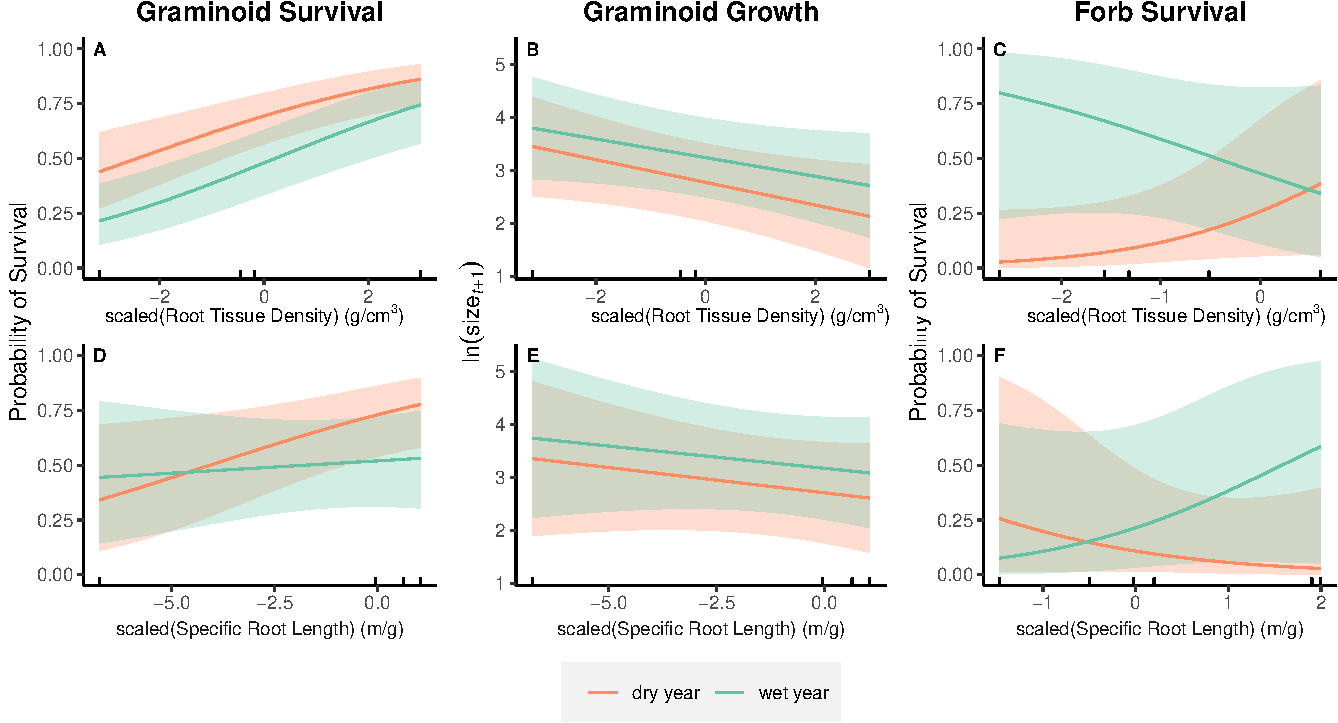
\includegraphics[width=.8\textwidth]{suppObservationsFig-1.pdf}
\caption{\internallinenumbers\small{
Illustration of the interaction between trait and SPEI for forb survival and graminoid survival and growth models for root tissue density and specific root length, which were not included in Fig. \ref{fig:PredsObs}. (\textbf{A}) There is not a signficant interactive effect of SPEI and RTD on graminoid survival. (\textbf{D}) There is a slightly significant interaction between SPEI and SRL that affects graminoid survival, although this model has a small $\Delta$ AIC value (Marg. R$^2$ = 0.60, Cond. R$^2$ = 0.67; interaction coef. = 0.01, \textit{P}$<$ 0.05). (\textbf{B, E}) Graminoid size$_\textit{t+1}$ is not significantly affected by an interaction between SPEI and RTD or SPEI and SRL. (\textbf{C, F}) Forb survival is significantly affected by an interaction between RTD and SPEI (Marg. R$^2$ = 0.05, Cond. R$^2$ = 0.42; interaction coef. = -0.41, \textit{P}$<$ 0.01) and between SRL and SPEI (Marg. R$^2$ = 0.03, Cond. R$^2$ = 0.61; interaction coef. = 0.39, \textit{P}$<$ 0.01), although both of these models have small $\Delta$ AIC values.
}}
\label{fig:GramSurv_all}
\end{figure}



\end{document}